\chapter{Polar Integration}
\label{chap:polar-integration}

\section{Area Bounded by Polar Curve}
\label{sec:area-bounded-by-polar-curve}

\begin{figure}[H]
  \centering
  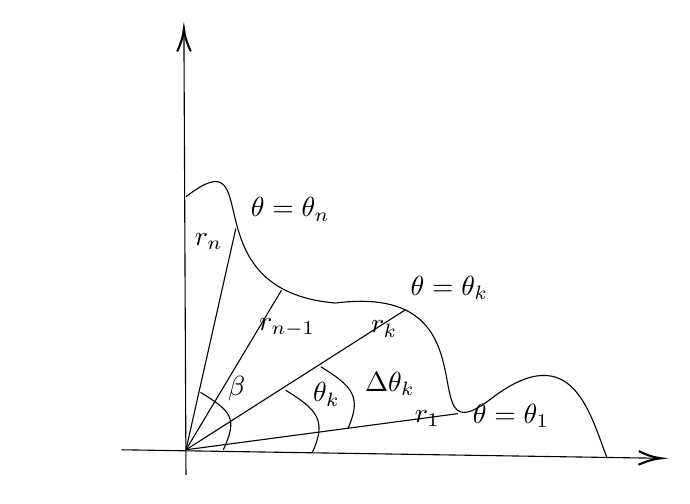
\begin{tikzpicture}[x=0.75pt,y=0.75pt,yscale=-1,xscale=1]
%uncomment if require: \path (0,231); %set diagram left start at 0, and has height of 231

%Straight Lines [id:da06955700187529645] 
    \draw    (198,219) -- (197.01,6) ;
    \draw [shift={(197,4)}, rotate = 89.73] [color={rgb, 255:red, 0; green, 0; blue, 0 }  ][line width=0.75]    (10.93,-3.29) .. controls (6.95,-1.4) and (3.31,-0.3) .. (0,0) .. controls (3.31,0.3) and (6.95,1.4) .. (10.93,3.29)   ;
%Straight Lines [id:da9321983324898755] 
    \draw    (167,206.87) -- (425,210.94) ;
    \draw [shift={(427,210.97)}, rotate = 180.9] [color={rgb, 255:red, 0; green, 0; blue, 0 }  ][line width=0.75]    (10.93,-3.29) .. controls (6.95,-1.4) and (3.31,-0.3) .. (0,0) .. controls (3.31,0.3) and (6.95,1.4) .. (10.93,3.29)   ;
%Curve Lines [id:da1148066759577353] 
    \draw    (198,84.94) .. controls (238,54.2) and (198,130.02) .. (270,136.17) ;
%Curve Lines [id:da25400979628298026] 
    \draw    (270,136.17) .. controls (350,125.93) and (305,213.02) .. (345,182.28) ;
%Curve Lines [id:da3491165874349259] 
    \draw    (345,182.28) .. controls (385,151.54) and (393,191.5) .. (401,210.97) ;
%Straight Lines [id:da5518412714711063] 
    \draw    (222,100.31) -- (198,206.87) ;
%Straight Lines [id:da6744383330094643] 
    \draw    (329,189.45) -- (198,206.87) ;
%Straight Lines [id:da5280623951078585] 
    \draw    (304,139.25) -- (198,206.87) ;
%Straight Lines [id:da6376375650592273] 
    \draw    (244,130.02) -- (198,206.87) ;
%Curve Lines [id:da7246741803143028] 
    \draw    (205,179.2) .. controls (220,188.43) and (223,191.5) .. (216,206.87) ;
%Curve Lines [id:da5230971502499104] 
    \draw    (263,166.91) .. controls (278,176.13) and (283,181.25) .. (276,196.62) ;
%Curve Lines [id:da014511263591748036] 
    \draw    (246,178.18) .. controls (261,187.4) and (266,192.52) .. (259,207.89) ;

% Text Node
    \draw (217,170.22) node [anchor=north west][inner sep=0.75pt]   [align=left] {$\displaystyle \beta $};
% Text Node
    \draw (283,168.17) node [anchor=north west][inner sep=0.75pt]   [align=left] {$\displaystyle \Delta \theta _{k}$};
% Text Node
    \draw (258,173.29) node [anchor=north west][inner sep=0.75pt]   [align=left] {$\displaystyle \theta _{k}$};
% Text Node
    \draw (335,183.54) node [anchor=north west][inner sep=0.75pt]   [align=left] {$\displaystyle \theta =\theta _{1}$};
% Text Node
    \draw (228,84.15) node [anchor=north west][inner sep=0.75pt]   [align=left] {$\displaystyle \theta =\theta _{n}$};
% Text Node
    \draw (307,186.61) node [anchor=north west][inner sep=0.75pt]   [align=left] {$\displaystyle r_{1}$};
% Text Node
    \draw (286,143.58) node [anchor=north west][inner sep=0.75pt]   [align=left] {$\displaystyle r_{k}$};
% Text Node
    \draw (122,137) node [anchor=north west][inner sep=0.75pt]   [align=left] {$ $};
% Text Node
    \draw (201,101.57) node [anchor=north west][inner sep=0.75pt]   [align=left] {$\displaystyle r_{n}$};
% Text Node
    \draw (232,142.55) node [anchor=north west][inner sep=0.75pt]   [align=left] {$\displaystyle r_{n-1}$};
% Text Node
    \draw (305,122.06) node [anchor=north west][inner sep=0.75pt]   [align=left] {$\displaystyle \theta =\theta _{k}$};
  \end{tikzpicture}
  \caption{Area Bounded by Polar Curves}
  \label{fig:area-bounded-by-polar-curves}
\end{figure}

For the \(k^{th}\) sector the area of the sector is:
\[ A_{k} = \frac{1}{2} r_{k}^2\theta \]
Then the area of all the sectors is:
\[\sum_{k=1}^{n} A_{k}\]
Then replacing the summation with limit as \(n\to \infty\) then, the area
bounded by the curve is:
\[ A = \int_{\alpha}^{\beta}A_{k} \] 

\begin{remark}[Main Point]
  We need to know what the \(\alpha\) and \(\beta\) is.\\
  This type of integration is useful for finding the shared area by two curve.
\end{remark}

Think and visualize of a situation where there are two curves and we need to
find the area bounded by one curve but not the other.\\
Let's say that the curve that is the one we need to find the area bounded by it
is \(r=f(\theta)\) and the other one is \(r=g(\theta)\).

Then the area bounded by \(r=f(\theta)\) is:
\[ A_{f} = \int_{\alpha}^{\beta} \frac{1}{2} (f(\theta))^2 d\theta \] 
\[ A_{g} = \int_{\alpha}^{\beta} \frac{1}{2} (g(\theta))^2 d\theta \] 
Then, the area bounded by \(f\) but not \(g\) is:
\[ A = \int_{\alpha}^{\beta} f(\theta)^2 - g(\theta)^2 d\theta \]
